\documentclass[11pt,a4paper]{article}

\usepackage[utf8]{inputenc}
\usepackage[T1]{fontenc}
\usepackage{lmodern}
\usepackage[margin=1in]{geometry}
\usepackage{amsmath}
\usepackage{graphicx}
\usepackage{booktabs}
\usepackage{tabularx}
\usepackage{caption}
\usepackage{enumitem}
\usepackage{microtype}
\usepackage[hidelinks]{hyperref}
\usepackage{xurl}

\captionsetup{font=small,labelfont=bf}
\setlist{itemsep=2pt,topsep=4pt}
\setlength{\emergencystretch}{1.5em}

\title{\textbf{Synaptic: Agents Propose, Code Decides}\\[4pt]
\large Honest trend detection in NASA Earth data with a pre-registered AI research group}

\author{Nassim Abouelfadile \and Reda Louriki\\[4pt]
\normalsize Team Synaptic, Casablanca, Morocco\\
\normalsize NASA Space Apps Challenge 2026 --- \emph{Be an Earth System Trend Detective!}}

\date{November 2026}

\begin{document}
\maketitle

\begin{abstract}
A line drawn through Earth observation data is easy to over-read. Year-to-year memory in climate series makes
ordinary trend tests call chance ``significant'', and testing many ideas guarantees that some pass by luck. We present
\emph{Synaptic}, which answers this problem at two levels. \emph{Trend Detective} is an application that lets anyone
choose one of 41 NASA variables, any region and any period, and returns the time series with a verdict in plain
words, computed with tests that account for carry-over between years. Behind it, an AI research group of NVIDIA
Nemotron agents searches NASA data for changes, but no agent can promote its own claim: every hypothesis carries a
confirmation test written down before its data are downloaded, and code runs that test on data the agents never saw.
Applied to NASA data, the system (i) re-tested the river-mouth chlorophyll trends of a NASA reference study and did not
detect them in 24 years of MODIS once carry-over is accounted for ($p = 0.37$--$0.43$); (ii) measured that the
winter 2025--26 rains in northern Morocco added 17--21\,km$^3$ of water storage, confirmed on a second satellite, SMAP
($p = 0.011$, below a pre-set threshold of 0.0167); (iii) measured the largest seasonal water gains since 2003 around
Lake Chad (about 75\,km$^3$) and in the central Sahara (46--73\,km$^3$) after the 2024 rains; and (iv) found that when
the United Arab Emirates moved its weekend in 2022, the day with the cleanest air over Dubai and Abu Dhabi moved from
Friday to Sunday ($p = 0.00005$). Of 81 pre-registered tests, most came back ``not shown'', and we report them all.
\end{abstract}

% ---------------------------------------------------------------------------------------------------------------
\section{Introduction}

NASA publishes decades of free satellite and model data about the Earth system. The 2026 Space Apps challenge
\emph{Be an Earth System Trend Detective} asks for a tool that lets anyone choose a variable, a region and a period,
build the time series, and test whether its trend is statistically significant. The difficulty is not drawing the
line; it is deciding honestly whether the line means anything. Three things routinely mislead:

\begin{enumerate}
  \item \textbf{Noisy years.} A single wet, hot or smoky year can tilt a short record.
  \item \textbf{Hidden memory.} Climate series remember the previous year (soil water, ocean heat, slow cycles).
        Standard tests assume independent years and therefore report trends that are not there. In our own
        experiments on synthetic data, carry-over alone made 35\% of pure-noise grid cells ``significant'' before
        correction.
  \item \textbf{Too many tries.} An automated search that tests hundreds of regions and variables will always find
        something with $p < 0.05$.
\end{enumerate}

Recent work has shown that teams of large-language-model agents can carry out real scientific search, for example
in genome mining \cite{yoon2026} and hypothesis generation for biomedicine \cite{gottweis2026}. Such systems are
powerful, but they also amplify the third problem: an agent that runs many analyses and is rewarded for finding
something will over-claim. Synaptic adapts the multi-agent design of Yoon et al.\ \cite{yoon2026} to Earth
observation and adds one rule that shapes everything else: \textbf{agents propose, code decides.}

Our contributions are:
\begin{itemize}
  \item an open application for the challenge's five steps, with statistics that account for carry-over and a
        verdict in plain language, cross-checked against NASA Giovanni;
  \item an agentic research workflow in which hypotheses are pre-registered in git, confirmation data are held out
        from the agents, and verdicts can only be raised by code;
  \item four results on NASA data, each with its test registered before its data were downloaded, and a full
        account of what was tested and not shown.
\end{itemize}

% ---------------------------------------------------------------------------------------------------------------
\section{Trend Detective: the application}

Figure~\ref{fig:app} shows the user's path. The user chooses (1) a variable from 41 monthly NASA variables, described
in plain language: MERRA-2 reanalysis fields, MODIS Aqua aerosol, cloud, sea surface temperature and chlorophyll,
OMI nitrogen dioxide and ozone, AIRS temperature at four heights, GPM IMERG rainfall, GLDAS land variables, CERES
radiation and GRACE/GRACE-FO water storage; (2) a region: any country, US state, a box or the whole world; and (3) a
period and season. The application fetches only that variable and region from NASA Earthdata Cloud (OPeNDAP and
Harmony subsetting), then (4) draws the yearly and monthly time series and a map of where the variable changes, and
(5) tests significance.

\begin{figure}[t]
  \centering
  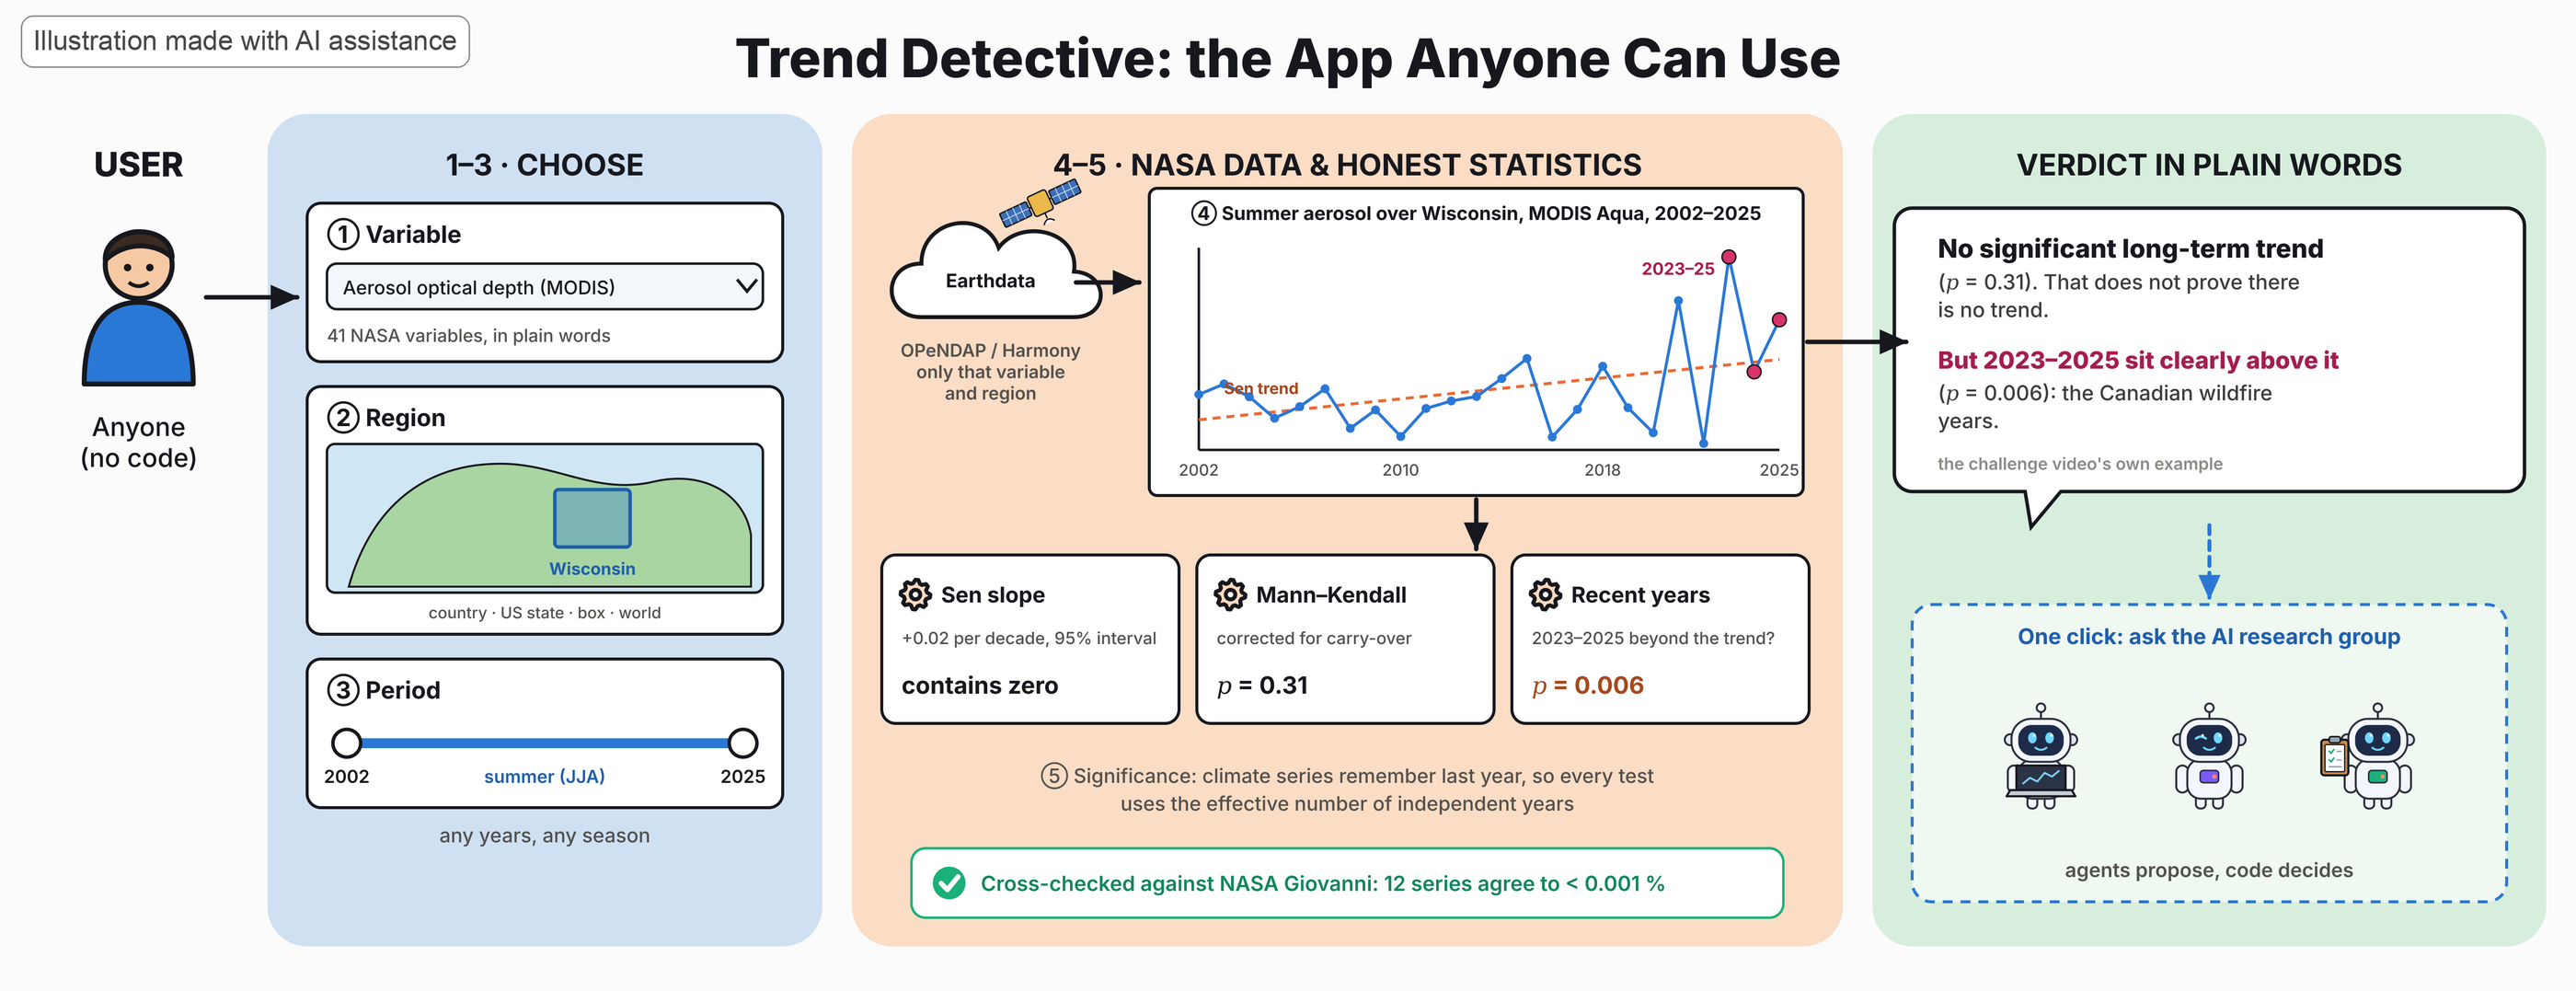
\includegraphics[width=\linewidth]{figures/fig_app.png}
  \caption{Trend Detective. The user chooses a variable, a region and a period; the application downloads only that
  data, draws the series and gives a verdict in plain words. The example is the challenge video's own case, summer
  aerosol over Wisconsin. One click hands the question to the AI research group. (Illustration made with AI assistance.)}
  \label{fig:app}
\end{figure}

\paragraph{Statistics that do not over-claim.} The trend is estimated with the Sen slope \cite{sen1968} and tested
with the Mann--Kendall test \cite{mann1945,kendall1975}. Because climate series carry memory from one year to the
next, the test variance is inflated by the long-run factor of a first-order autoregressive process fitted to the
detrended series (lag-1 autocorrelation, bias-corrected, with a regional floor). The application reports the
effective number of independent years and a 95\% interval for the slope. A separate test asks whether the latest
years sit beyond the trend, so that one record event is not mistaken for a trend. The verdict is written in words, for
example: \emph{``No significant trend ($p = 0.31$). That does not prove there is no trend; the change is not
distinguishable from year-to-year variability with this many years.''} For the challenge video's example, summer
aerosol optical depth over Wisconsin (MODIS Aqua, 2002--2025), the long-term trend is $+0.02$ per decade and not
significant ($p = 0.31$), while 2023--2025 sit clearly above it ($p = 0.006$): the Canadian wildfire years.

\paragraph{Checked against NASA's own tool.} Twelve monthly series fetched through the application and through NASA
Giovanni agree to better than 0.001\%. Finished analyses are saved, so examples answer offline.

% ---------------------------------------------------------------------------------------------------------------
\section{The agentic workflow}

\begin{figure*}[t]
  \centering
  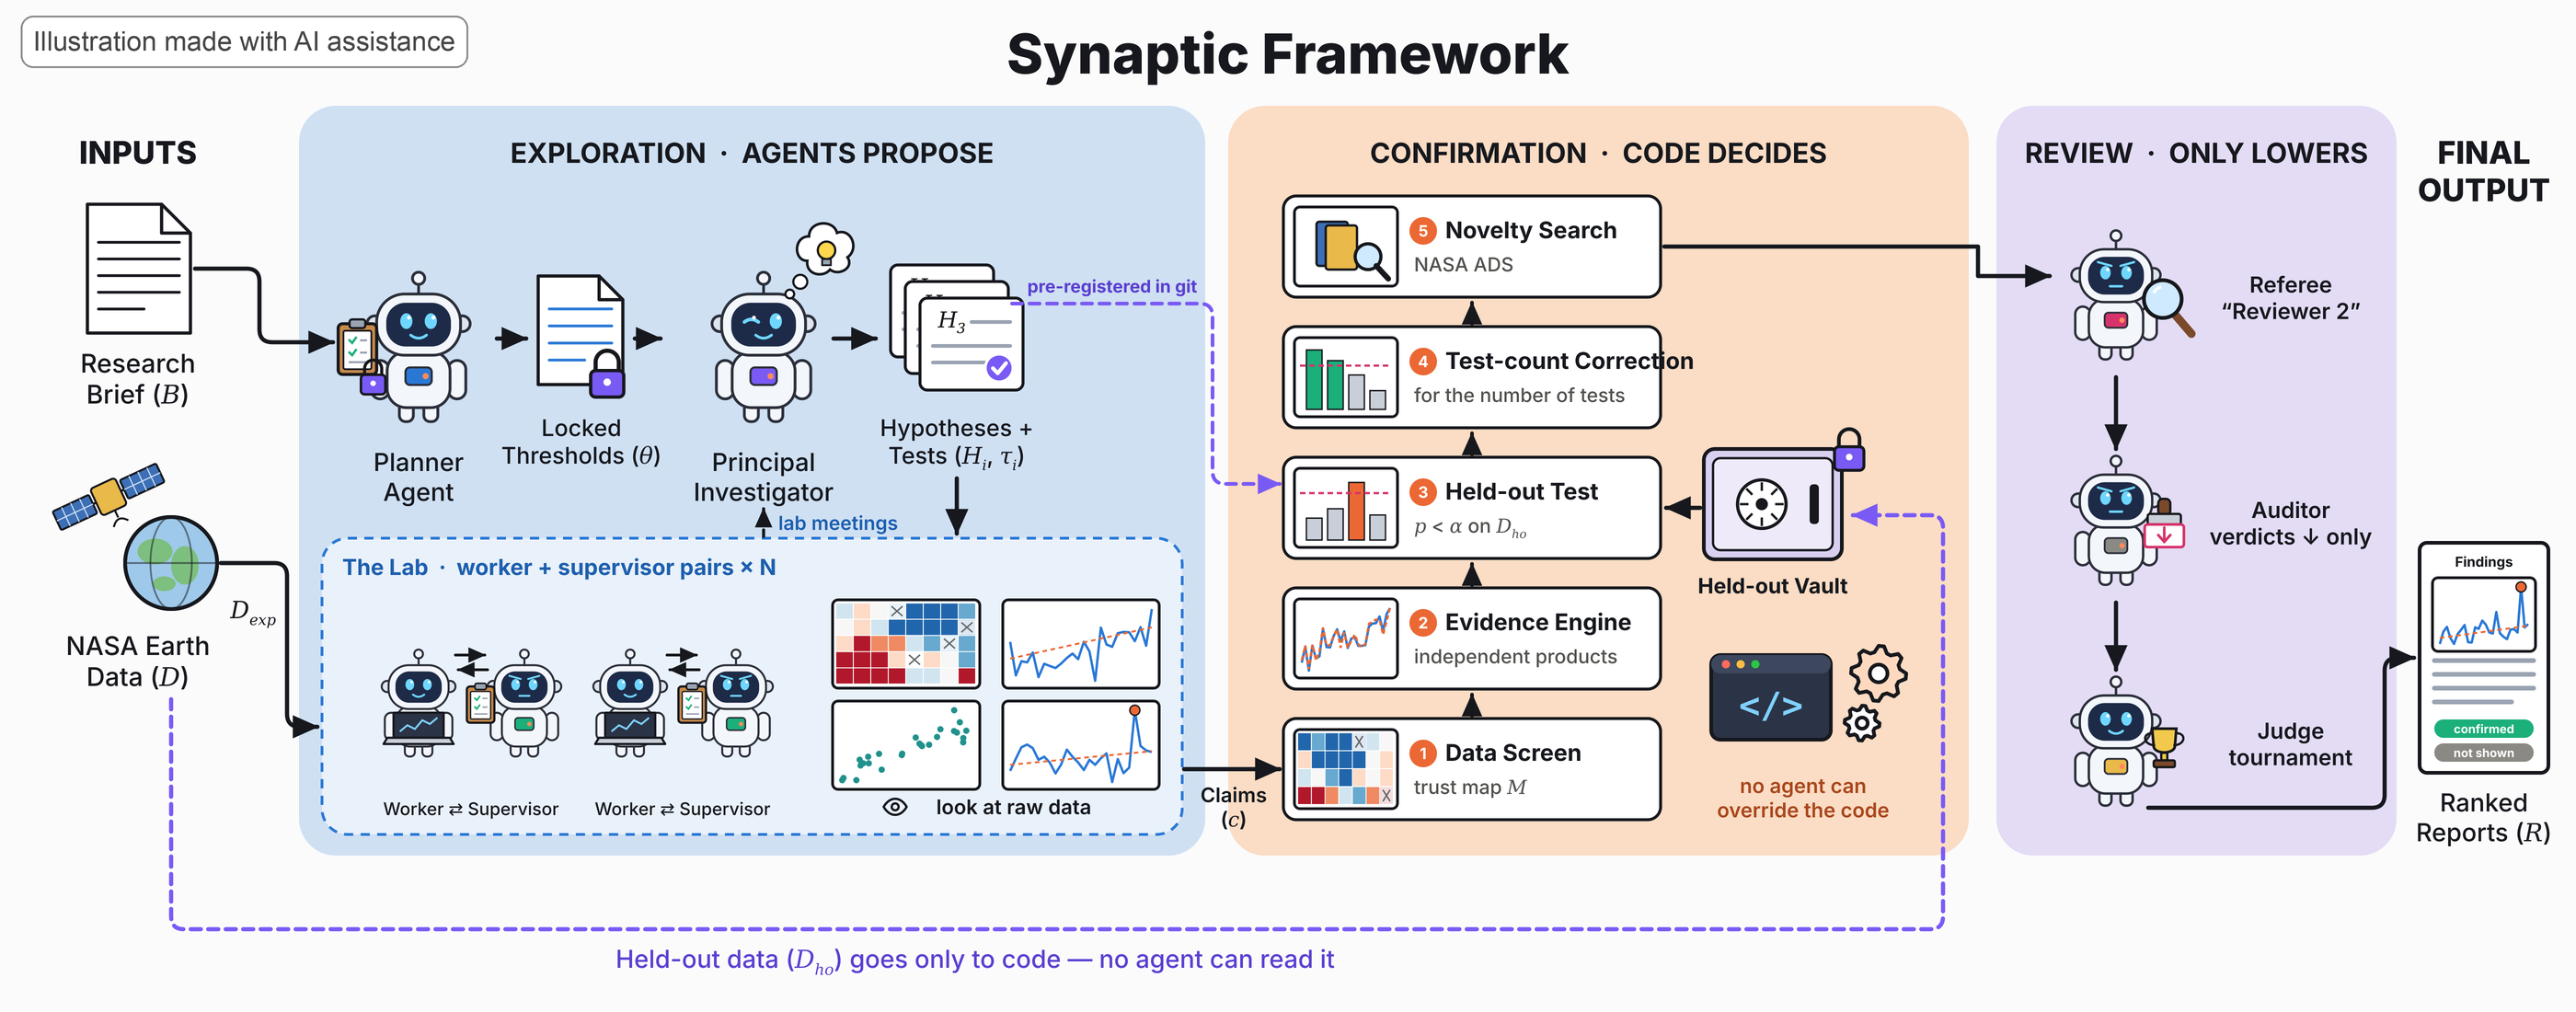
\includegraphics[width=\linewidth]{figures/fig_framework.png}
  \caption{The Synaptic framework. Agents explore the data they are allowed to see ($D_{exp}$) and propose
  hypotheses with tests written first. Code runs the confirmation gates on held-out data ($D_{ho}$) that no agent can
  read. Review agents can only lower a verdict. (Illustration made with AI assistance.)}
  \label{fig:framework}
\end{figure*}

\subsection{Roles}
Synaptic organises language-model agents as a small research group (Figure~\ref{fig:framework}). A campaign starts
from a \emph{research brief} written by the team: an open question, the region, the variables the agents may explore
and the datasets reserved for confirmation.

\begin{description}[leftmargin=1.2em,style=nextline]
  \item[Planner.] Turns the brief into a plan and \emph{locks every threshold before any data is seen}.
  \item[Principal investigator (PI).] Reads a literature scan of the open problem and writes 10--16 falsifiable
        hypotheses, each with its confirmation test and kill criteria written first; the rest wait in a reserve pool.
  \item[The lab.] Worker and supervisor pairs run in parallel. Workers must \emph{look at the data}: raw numbers and
        figures are placed in the vision model's context, and a task cannot be finished without it. Supervisors
        review every plan and every result. \emph{Lab meetings} every few tasks drop dead ends, order deeper tests
        and promote hypotheses from the reserve.
  \item[Referees (``Reviewer 2'').] Recompute and attack every supported claim, with at least three real checks.
  \item[Auditor.] A sceptical agent that re-reads every claim before reports are written. It can only lower a
        verdict.
  \item[Editor and judge.] Write result reports and rank them in a tournament in which every pair is judged in
        both orders, to cancel position bias.
\end{description}

The judgement roles (PI, auditor, judge) run on NVIDIA Nemotron 3 Ultra; workers run on Nemotron 3.5 Super VL, which
can read figures. Agent code runs in a sandbox with no network and no credentials. All actions, plans, results and
verdicts are written to a shared record.

\subsection{Held-out data and pre-registration}
The central design choice is a separation between what agents can see and what decides. Two kinds of hold-out are
used. In a \emph{dataset hold-out}, whole products (for example GRACE water storage, IMERG rainfall or CERES radiation)
are removed from the agents' tools; agents explore other products and propose claims. In a \emph{time hold-out}, agents
see a product only up to a cut-off year (for example GRACE up to 2015) and code confirms on the later years.

Every confirmation test is fixed in advance: dataset, region, months, event years, direction and threshold. The
specification is committed to git and pushed before the confirmation data are downloaded, and the results are
appended afterwards with any deviation listed (Figure~\ref{fig:prereg}). For the SMAP check of northern Morocco, the
registration was pushed at 07:45 and the results appended at 07:54: nothing in the specification could change after
the data were seen.

\begin{figure}[t]
  \centering
  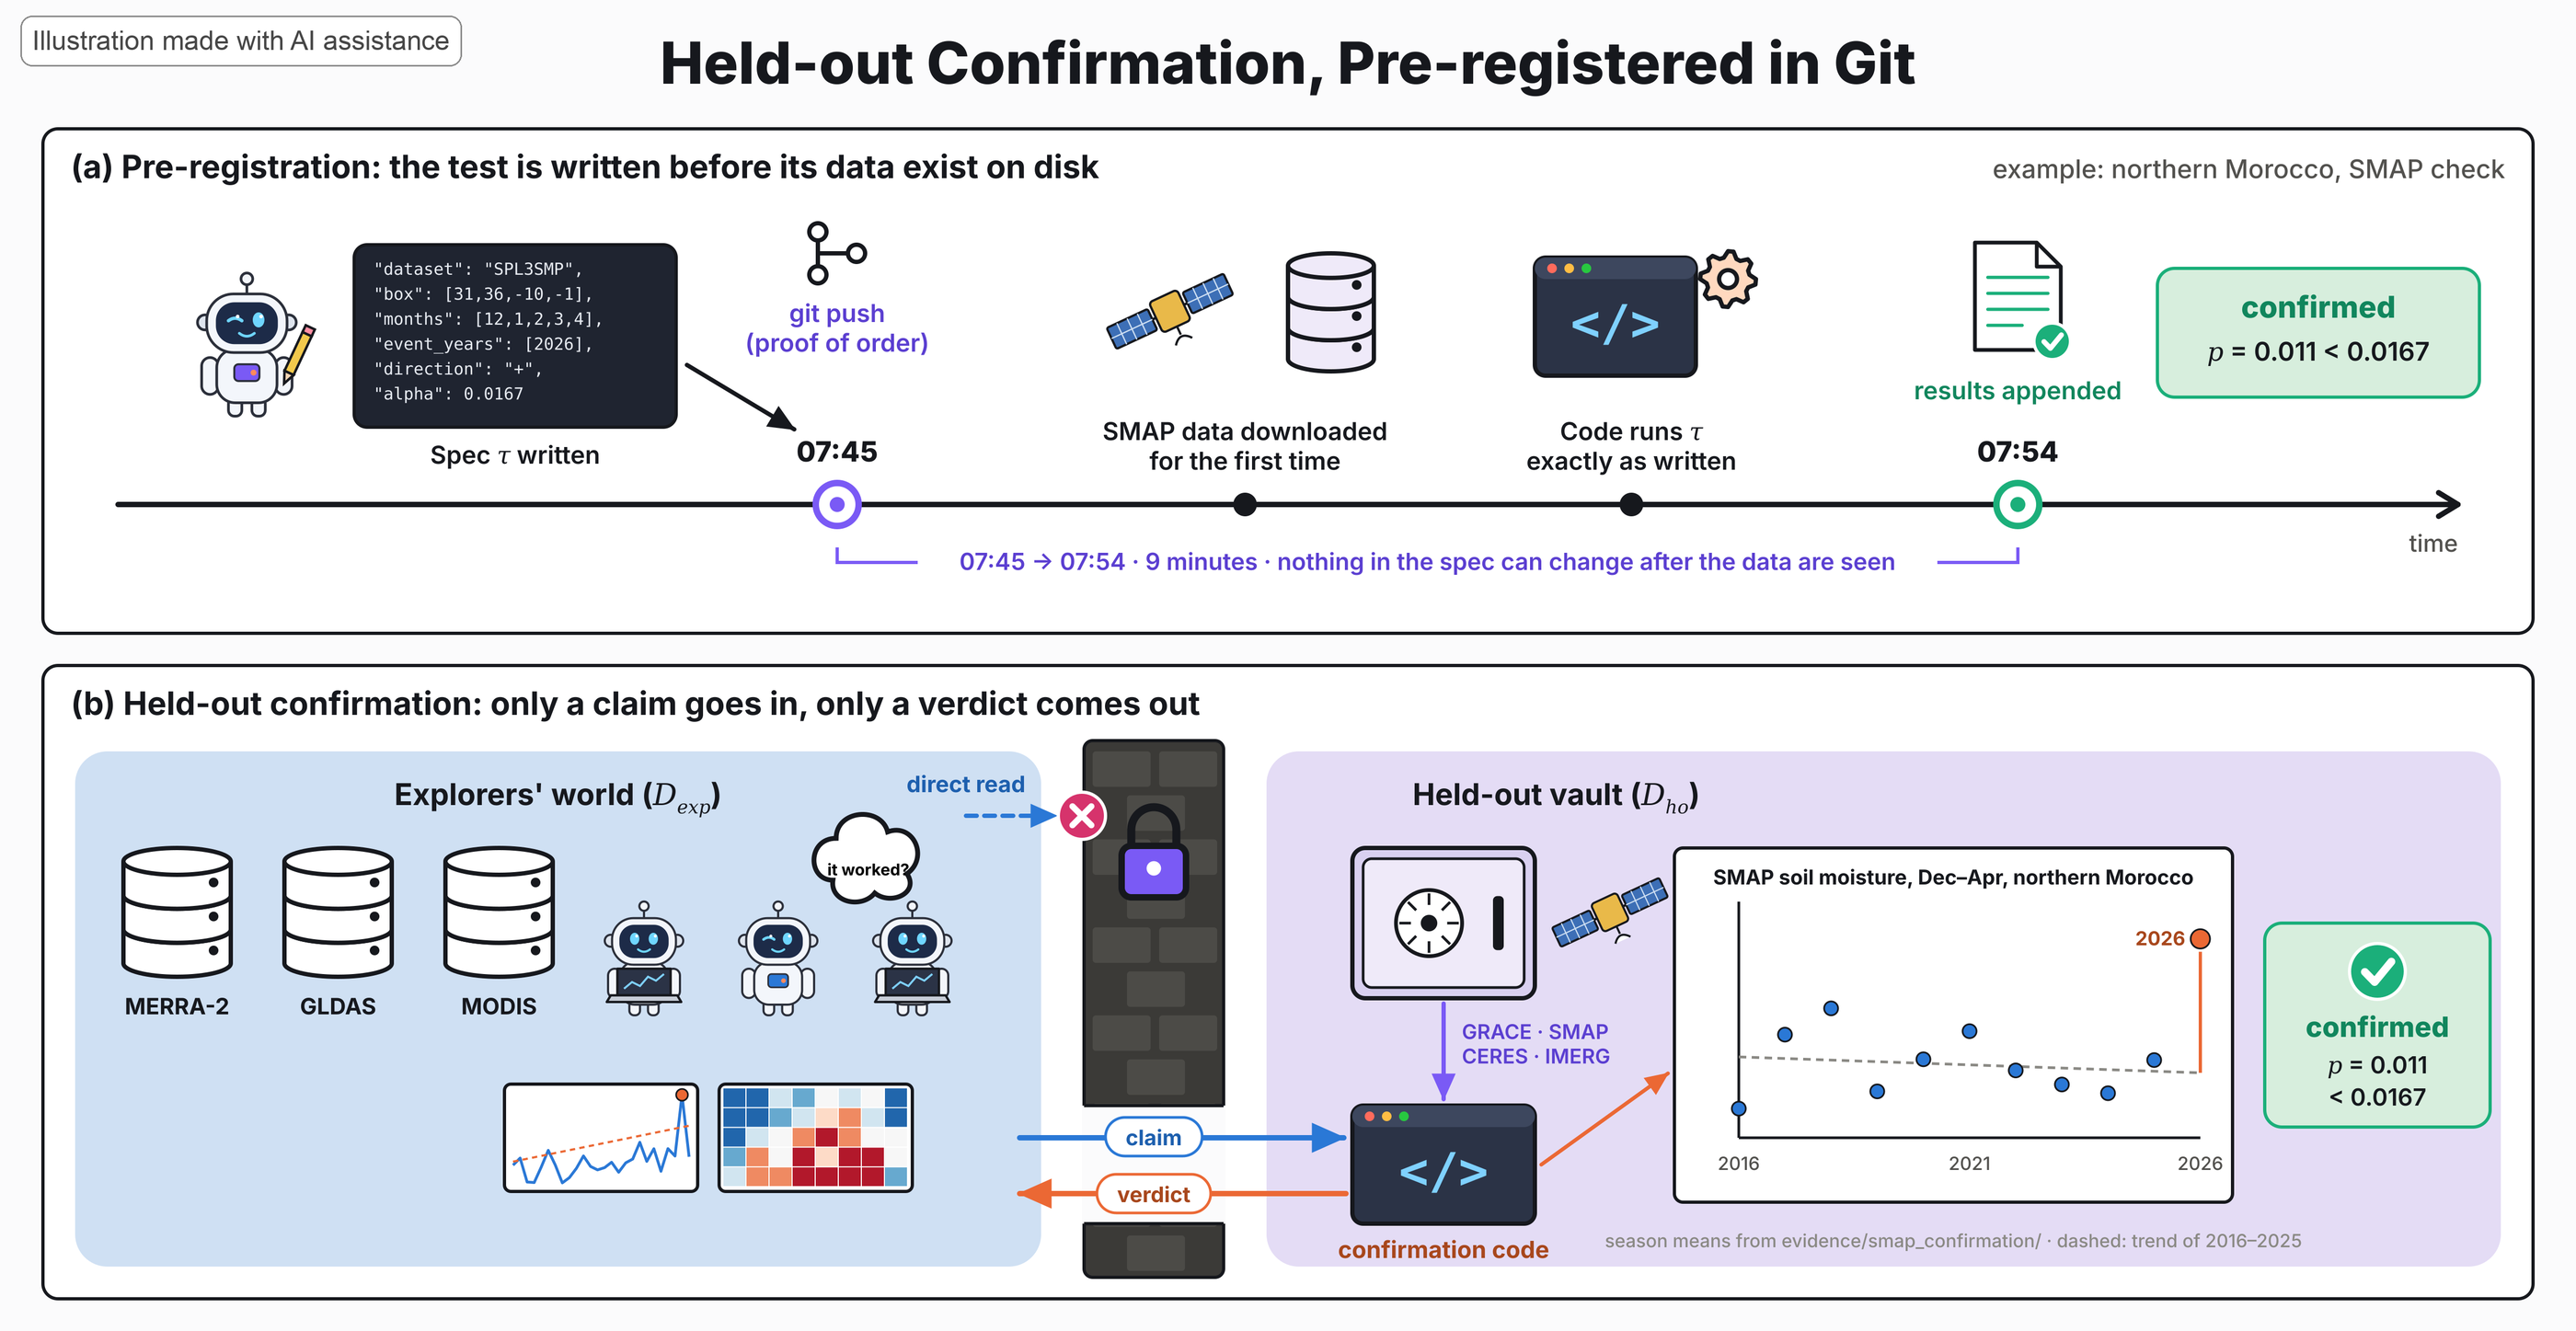
\includegraphics[width=\linewidth]{figures/fig_preregistration.png}
  \caption{Held-out confirmation, pre-registered in git. (a) The test specification is pushed before its data exist
  on disk. (b) Only a claim goes into the confirmation code and only a verdict comes out; agents cannot read the
  held-out data. The SMAP points are the real season means. (Illustration made with AI assistance.)}
  \label{fig:prereg}
\end{figure}

\subsection{Confirmation gates run by code}
A claim from the lab passes through five gates that no agent can override:
\begin{enumerate}
  \item \textbf{Data screen.} A trust map of every grid cell, comparing reanalysis with independent rainfall and
        temperature products, before any test.
  \item \textbf{Evidence engine.} The same statistic recomputed on independent products (for example GPCP, IMERG,
        Berkeley Earth, GLDAS), a robustness suite (leave-one-year-out, end points, without strong El Ni\~no years,
        block bootstrap) and field significance with spatial correlation preserved.
  \item \textbf{Held-out test.} The pre-registered test, run on data no agent has seen.
  \item \textbf{Correction for the number of tests.} A Bonferroni or Holm \cite{holm1979} threshold across the tests
        of a registration, plus a charge for earlier tests in the campaign.
  \item \textbf{Novelty check.} A NASA ADS literature search. Without a working search, novelty is reported as
        ``unverified'', never ``new''.
\end{enumerate}

\subsection{The evidence ladder and the verdict ratchet}
Every claim climbs the same ladder, and where it stops is what gets reported (Figure~\ref{fig:ladder}). A claim that
fails the held-out test or disagrees with a second dataset is \emph{not shown}. A non-significant result is absence of
evidence, so it is never labelled ``refuted''. A claim that passes but fails the correction is \emph{supported, not
confirmed}. A confirmed claim that is already published is \emph{known}. The verdict ratchet is enforced in code: only
the confirmation and novelty gates can move a claim up; referees, the auditor and follow-up tasks can only move it down.

\begin{figure*}[t]
  \centering
  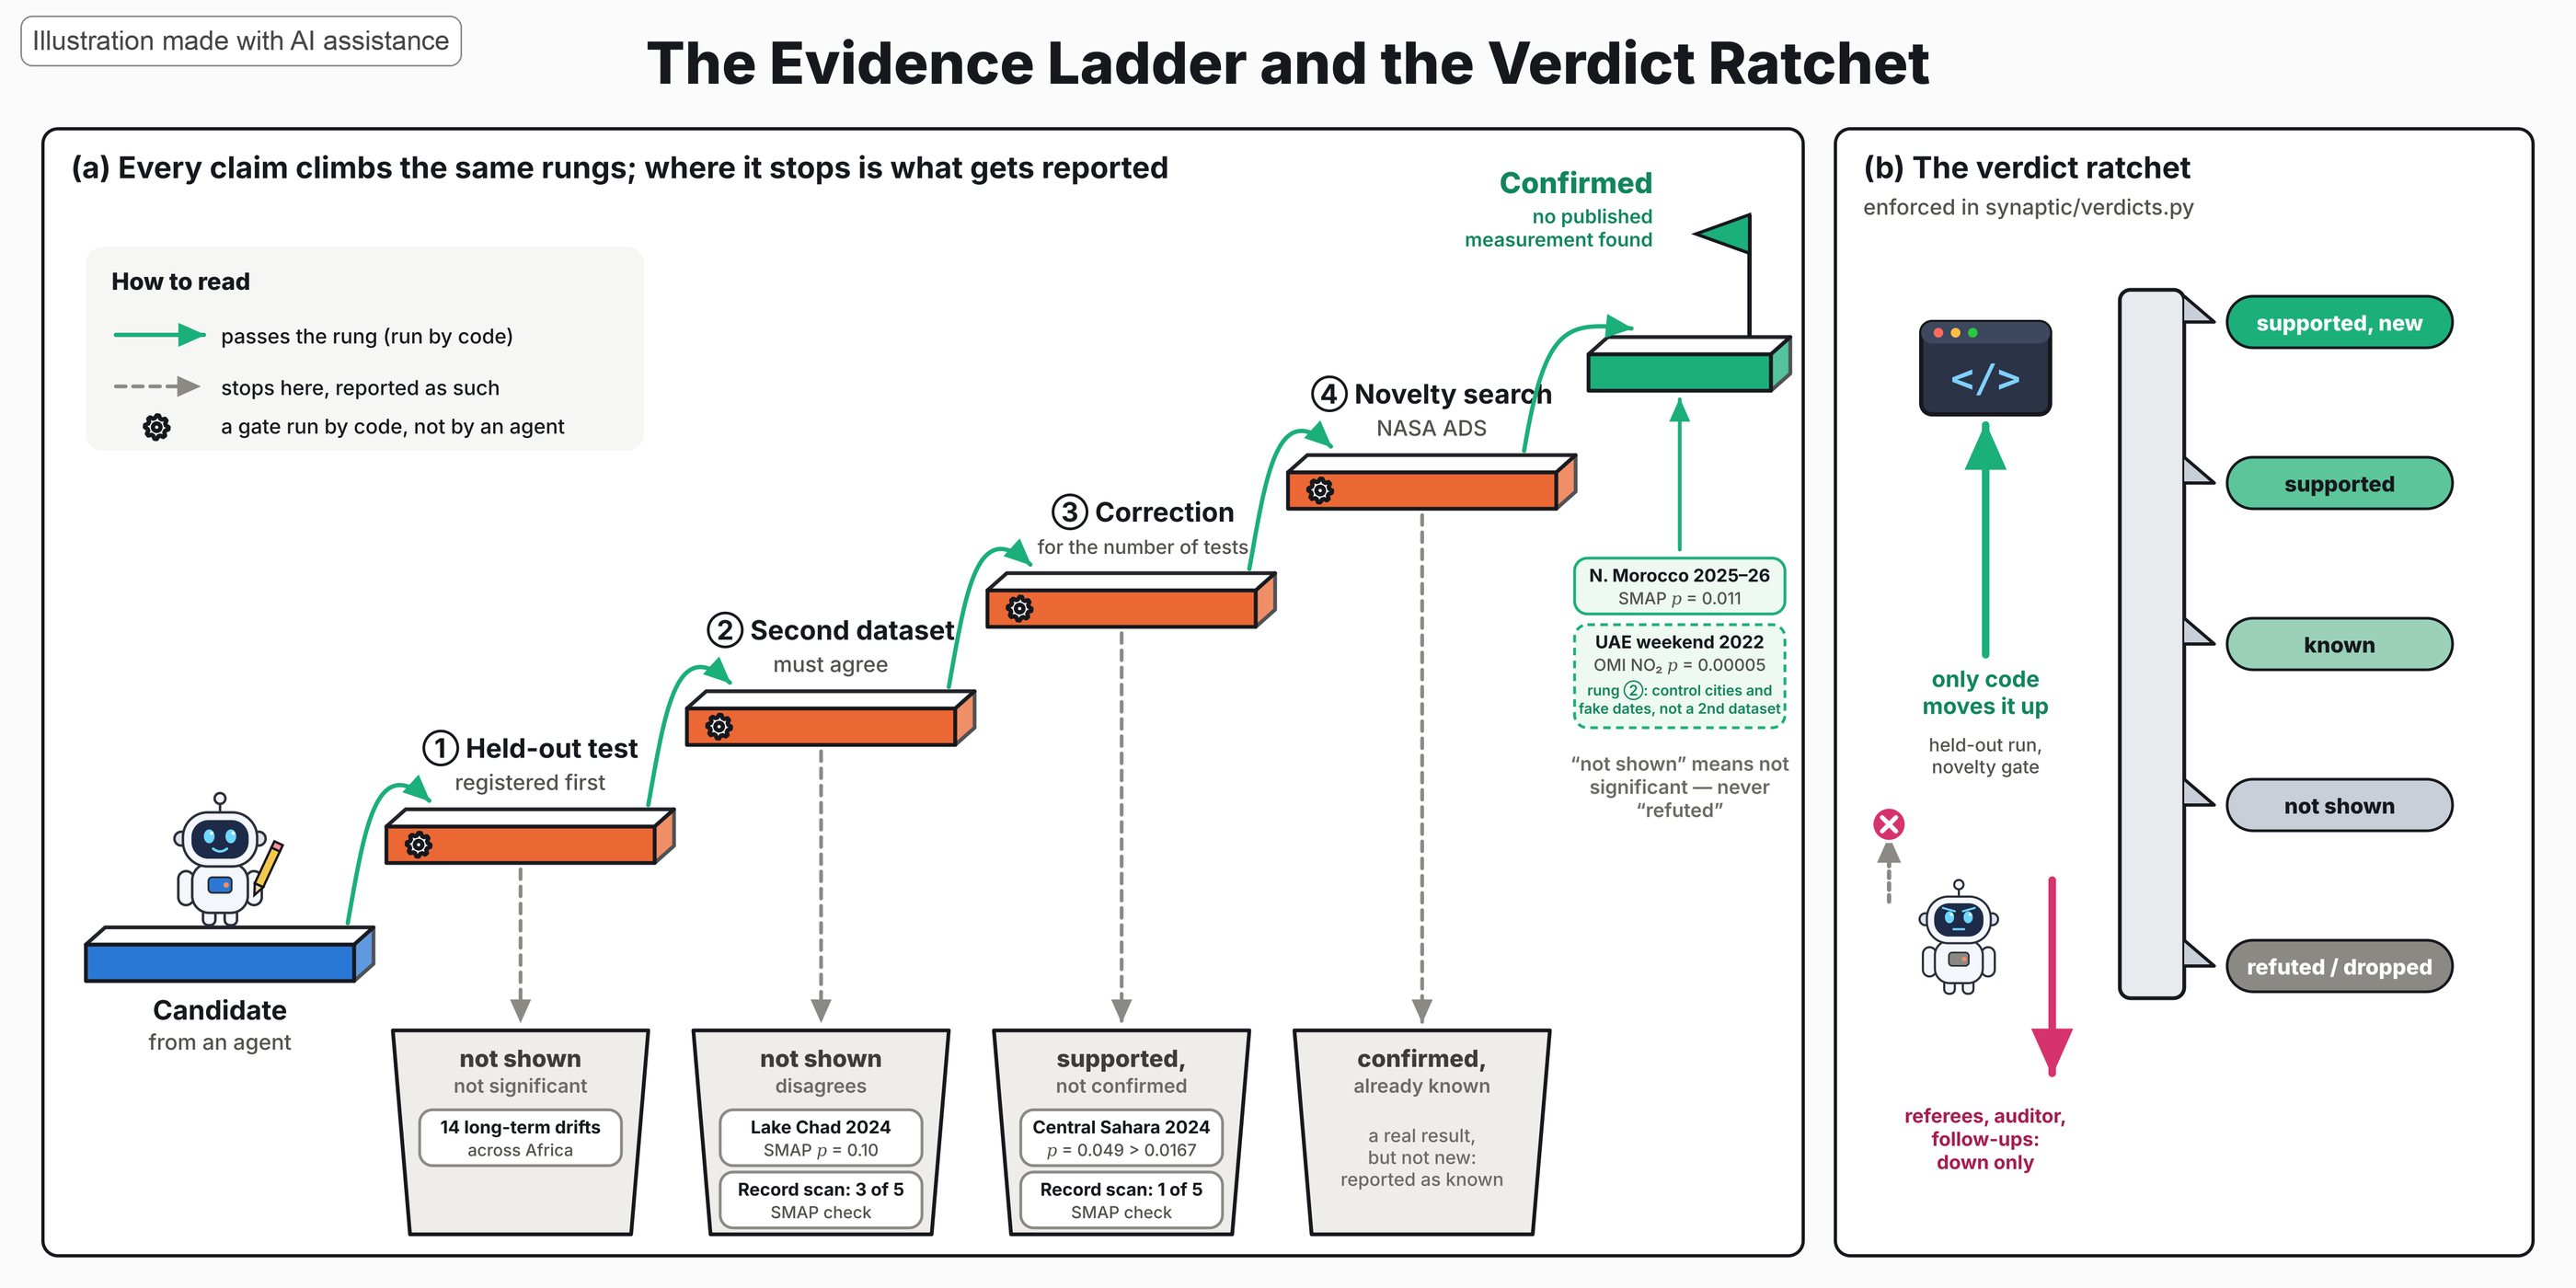
\includegraphics[width=\linewidth]{figures/fig_ladder.png}
  \caption{(a) The evidence ladder, with the real outcomes of our campaigns. (b) The verdict ratchet: only code moves a
  claim up. (Illustration made with AI assistance.)}
  \label{fig:ladder}
\end{figure*}

% ---------------------------------------------------------------------------------------------------------------
\section{Results}

Table~\ref{tab:results} summarises the four results. For each, we searched NASA ADS and found no published measurement
(results 2--4) or published re-test (result 1). We do not claim to be the first: we have not read every paper.

\begin{table}[t]
  \centering
  \small
  \begin{tabularx}{\linewidth}{@{}p{0.27\linewidth}X p{0.2\linewidth}@{}}
    \toprule
    Result & What the data show & Proof \\
    \midrule
    1. River-mouth chlorophyll (NASA reference study) & Three trends reported as significant (SeaWiFS 1998--2007)
      are not detected in MODIS 2002--2025 & $p = 0.37$--$0.43$; two code versions agree \\
    2. Northern Morocco, winter 2025--26 & 17--21\,km$^3$ more water stored than in a normal winter & SMAP check
      confirmed, $p = 0.011 < 0.0167$ \\
    3. Lake Chad basin and central Sahara, 2024 & About 75 and 46--73\,km$^3$; largest gains since 2003 & SMAP: not
      shown ($p = 0.10$); supported ($p = 0.049$) \\
    4. UAE weekend change, 2022 & Cleanest day in the air moved from Friday to Sunday & $p = 0.00005$; four control
      cities null \\
    \bottomrule
  \end{tabularx}
  \caption{Summary of results. All $p$-values come from tests registered before their data were downloaded.}
  \label{tab:results}
\end{table}

\subsection{A NASA reference study, re-tested}
The challenge resources include a NASA study of chlorophyll off river mouths (NTRS 20090042747) \cite{ntrs2009}, which
reported significant trends off the Mississippi (two sites, decreasing) and the Eel (increasing in summer) in SeaWiFS
data from 1998--2007. We re-tested the same boxes with MODIS Aqua 2002--2025 and a test that accounts for carry-over from
one month to the next. None of the three trends is detected (corrected $p = 0.43$, $0.40$ and $0.37$), and all three
MODIS slopes point the opposite way, though none is significant (Figure~\ref{fig:river}). The choice of test matters:
off Mississippi East, the 2002--2007 overlap with the original period is significant with the original method
($p = 0.004$) and not once carry-over is corrected ($p = 0.056$). One river, the Guadalquivir, shows a decrease of about
15\% per decade; a second satellite, VIIRS, does not yet confirm it ($p = 0.19$), so we report it as a lead. ``Not
detected'' means not significant over a different period and sensor; small trends are not excluded.

\begin{figure}[t]
  \centering
  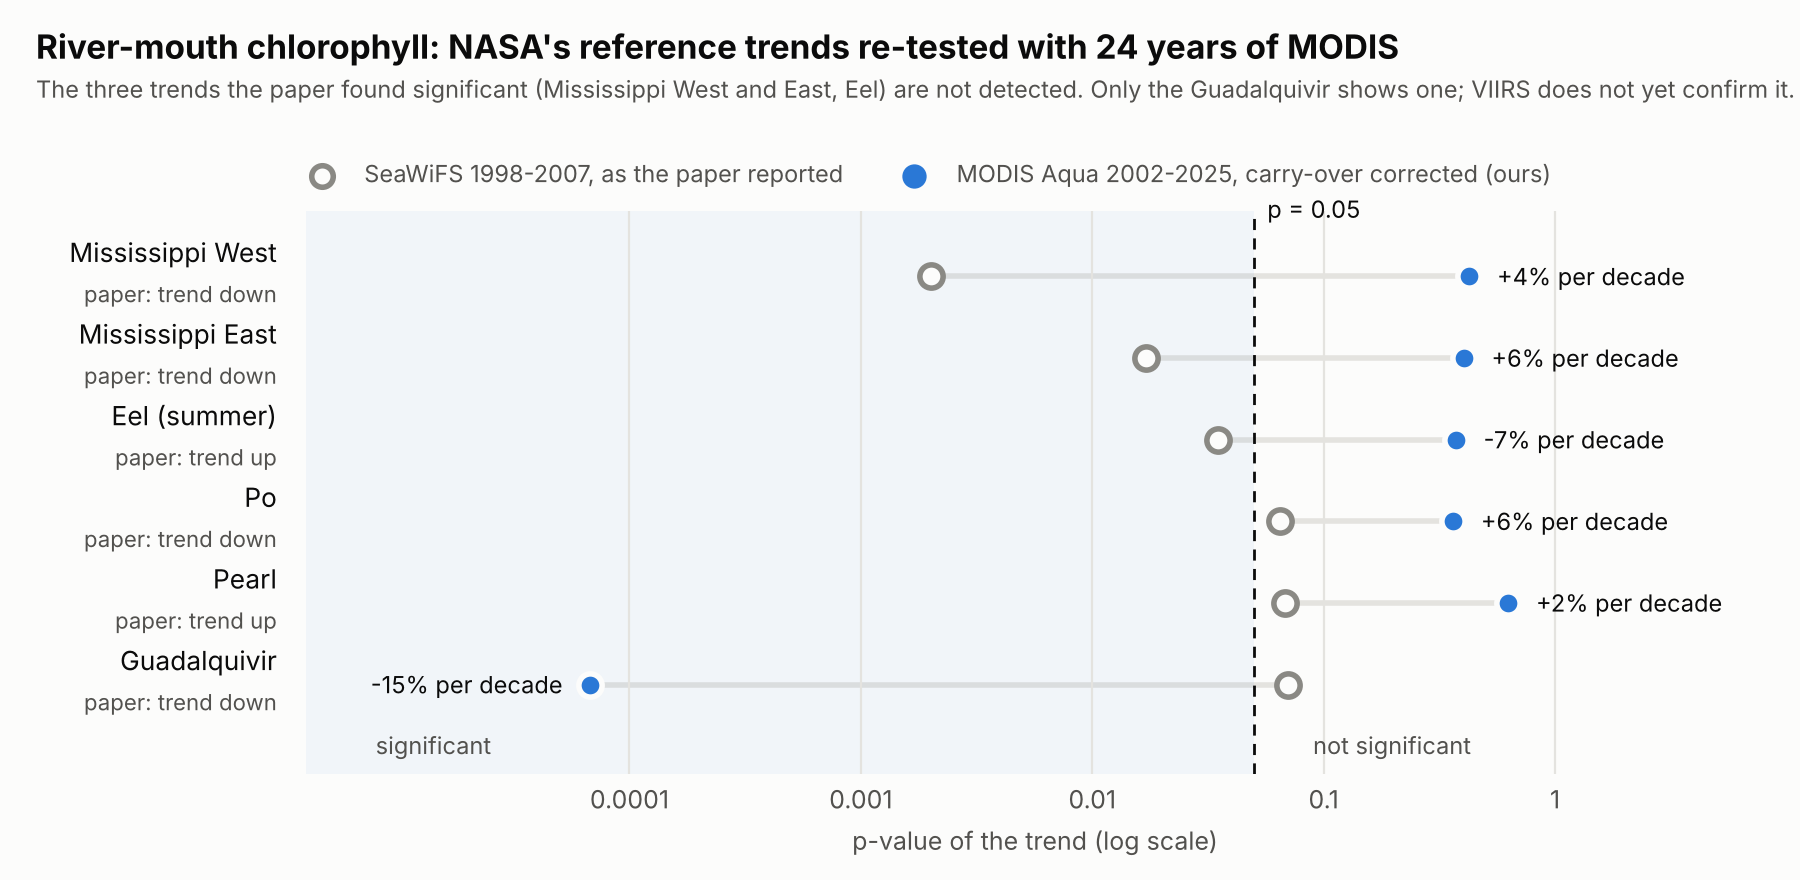
\includegraphics[width=\linewidth]{figures/river_pvalues.png}
  \caption{River-mouth chlorophyll: $p$-values reported by the NASA study versus our MODIS re-test.}
  \label{fig:river}
\end{figure}

\subsection{How much rain stayed in the ground}
NASA's GRACE and GRACE-FO satellites measure changes in Earth's gravity, which means they weigh the water stored in
soil, rivers, lakes and aquifers. For each region we computed the seasonal storage gain (end minus start of the wet
season), compared it with the mean gain of the other years, and converted the excess into a volume over the land
area, on two independently processed solutions: JPL mascons RL06.3 and NASA Goddard mascons RL06v2.0.

The 2024 rainy season added about 75\,km$^3$ of extra water in the Lake Chad basin (75 and 76\,km$^3$ on the two
solutions; Figure~\ref{fig:chad}) and 46--73\,km$^3$ in the central Sahara, the largest seasonal gains since 2003 in both
regions. About three quarters of the excess was still present seven months later, in the next dry season. In northern
Morocco, winter 2025--26, which ended a seven-year drought, added 17--21\,km$^3$, the second or third largest winter
gain since 2003.

\begin{figure}[t]
  \centering
  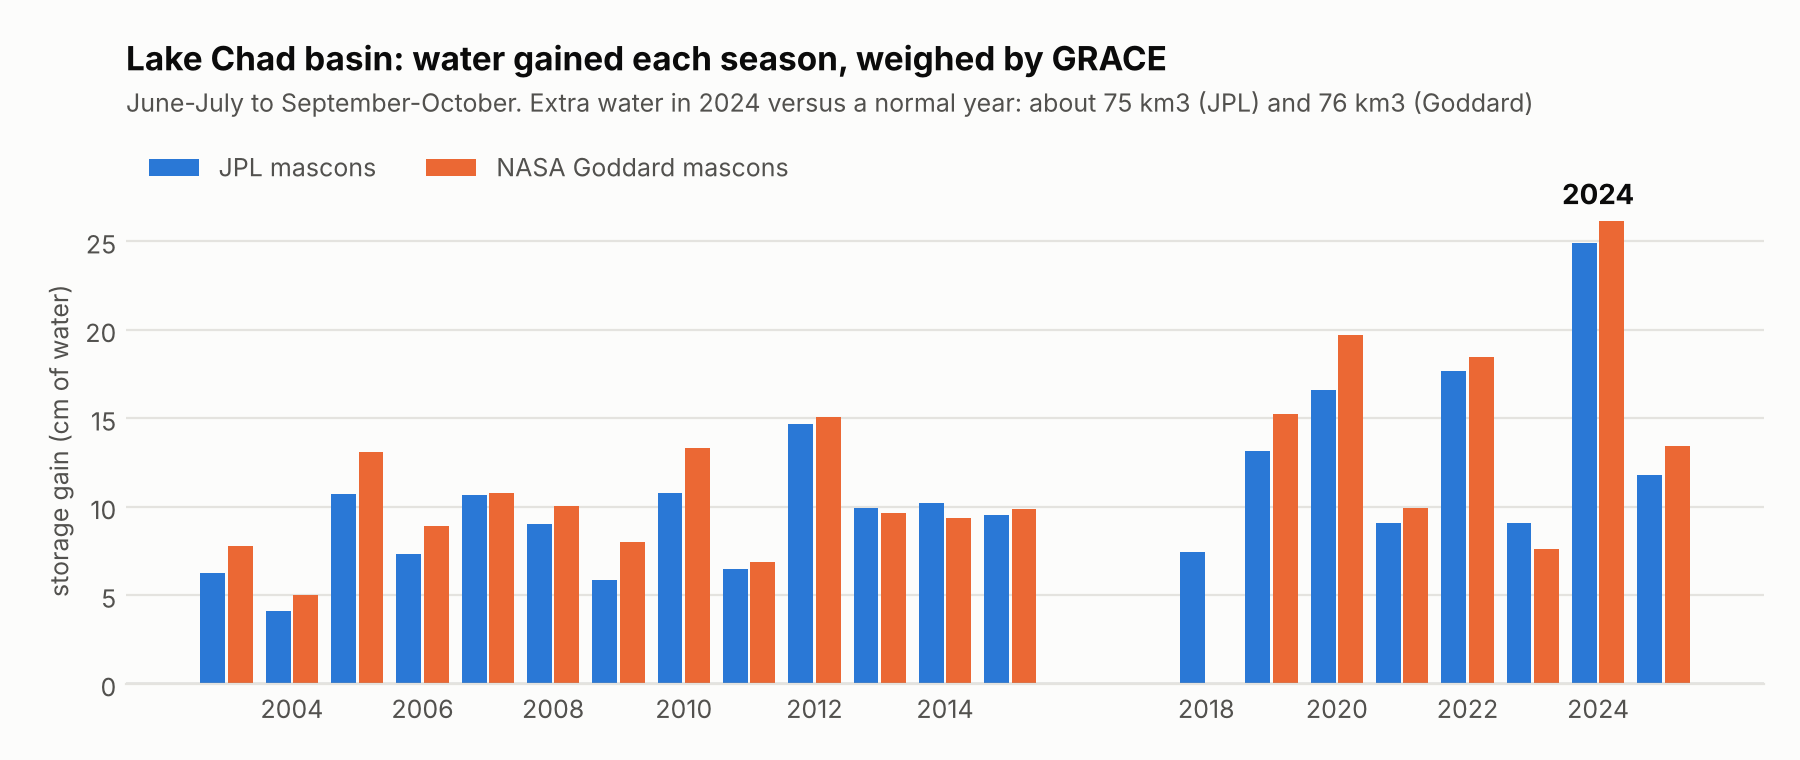
\includegraphics[width=\linewidth]{figures/A_lake_chad_grace_gains.png}
  \caption{Lake Chad basin: water gained each rainy season, weighed by GRACE on two independent solutions.}
  \label{fig:chad}
\end{figure}

These leads came out of 55 held-out tests, so their own $p$-values (0.002--0.013) do not survive a correction for the
number of tests. We therefore registered one fresh test per lead on an instrument never used in the project: NASA SMAP
L3 soil moisture, a microwave radiometer that shares no measurement, processing or science team with GRACE. The
statistic is the event season's departure from the linear trend of the other years, with carry-over accounted for, and
a lead is \emph{confirmed} only if $p < 0.05/3 = 0.0167$. Northern Morocco passed: 2026 is the wettest December--April
in SMAP's record, $+0.051$\,m$^3$/m$^3$ above the trend, $p = 0.011$ (Figure~\ref{fig:smap}). The central Sahara was
supported but not confirmed ($p = 0.049$) and Lake Chad was not shown ($p = 0.10$); with only 11 SMAP seasons, this test
is hard to pass. SMAP sees the top 5\,cm of soil, so it confirms that the land was unusually wet, not the volume.

\begin{figure}[t]
  \centering
  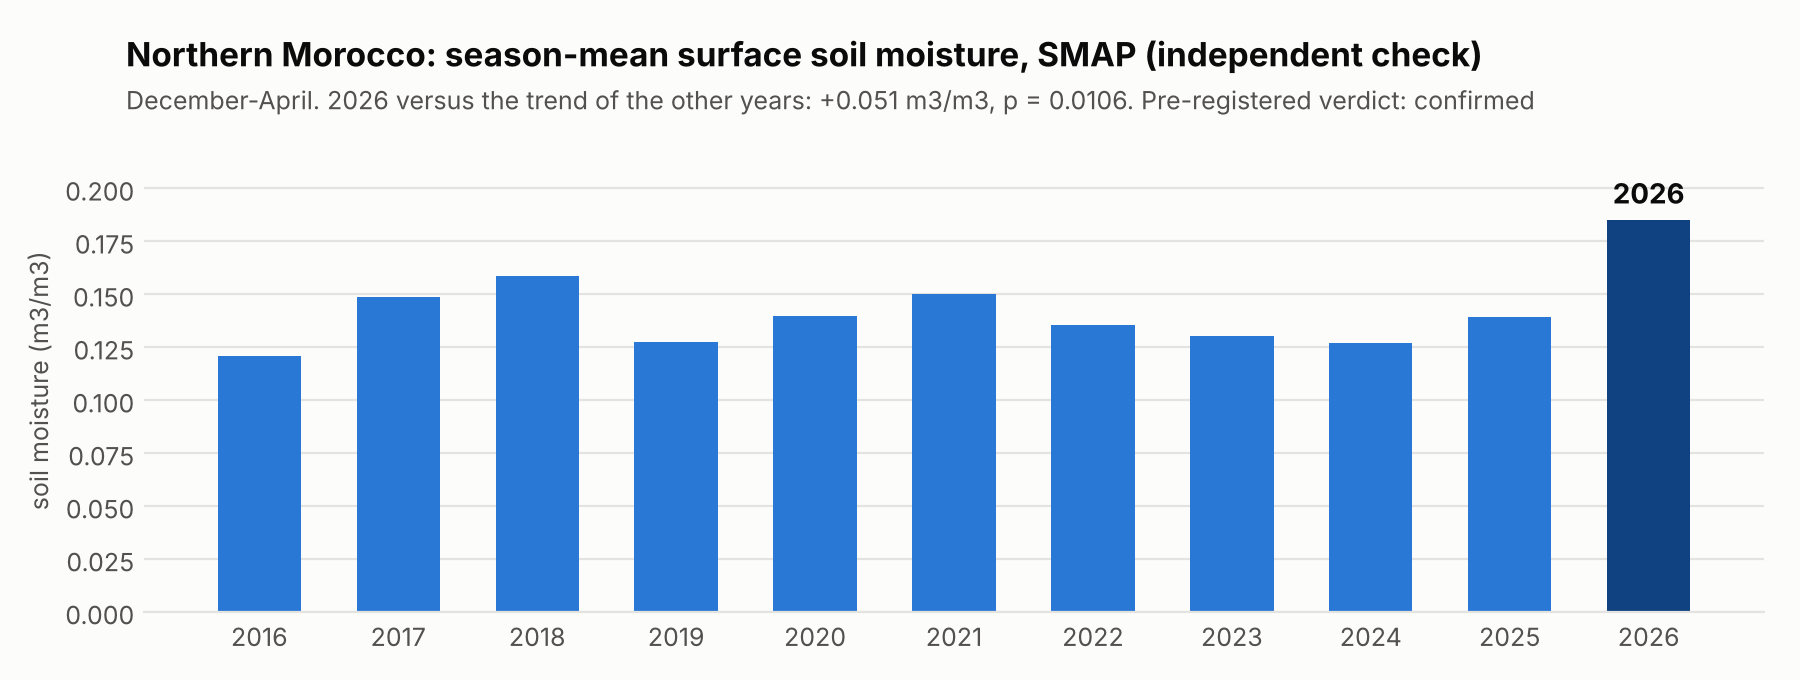
\includegraphics[width=\linewidth]{figures/C_north_morocco_smap.png}
  \caption{Northern Morocco: SMAP surface soil moisture, December--April. 2026 is the wettest season in the record.}
  \label{fig:smap}
\end{figure}

\subsection{A human-made change, seen from space}
The searches above look for something unusual and then need a second dataset. Our last registration ran the other way:
it started from dated facts on the ground. City nitrogen dioxide (NO$_2$), mostly from traffic, power and industry,
drops on rest days, and four countries moved their weekend on a known date within the record of NASA's OMI instrument.
For each city we used daily tropospheric NO$_2$ columns (OMNO2d v4, 0.25$^\circ$, October 2004 to October 2026, 8{,}017
days) averaged over a box of about 80\,km, and expressed each weekday relative to days that were working days both
before and after the change. The statistic $D$ is the change, from before to after, in the difference between the day
predicted to rise (it becomes a working day) and the day predicted to fall (it becomes a rest day), averaged over the
cities. Under the null hypothesis the before/after labels of whole weeks are exchangeable, so they are permuted 20{,}000
times; a Holm correction is applied across the four countries.

On 1 January 2022 the UAE moved its weekend from Friday--Saturday to Saturday--Sunday. Over Dubai and Abu Dhabi, Friday
went from 24\% below a working day to 5\% below, and Sunday went from 5\% below to 24\% below ($D = 0.38$,
$p = 0.00005$; Figure~\ref{fig:uae}). Each city shows it separately; Friday was 17--32\% below a working day in every
year from 2005 to 2021 and 3--10\% below from 2022 on. Control cities (Doha, Tehran, Cairo, Kuwait City) show nothing on
that date, fake change dates (2019, 2024) show nothing, and removing 2020 changes nothing. The same test passed for Oman
and Saudi Arabia (2013), but Kuwait City, whose weekend did not change in 2013, shifted by a similar amount, so we do not
rely on those two. This is a change in a weekly pattern, not a long-term trend and not a claim about emissions.

\begin{figure}[t]
  \centering
  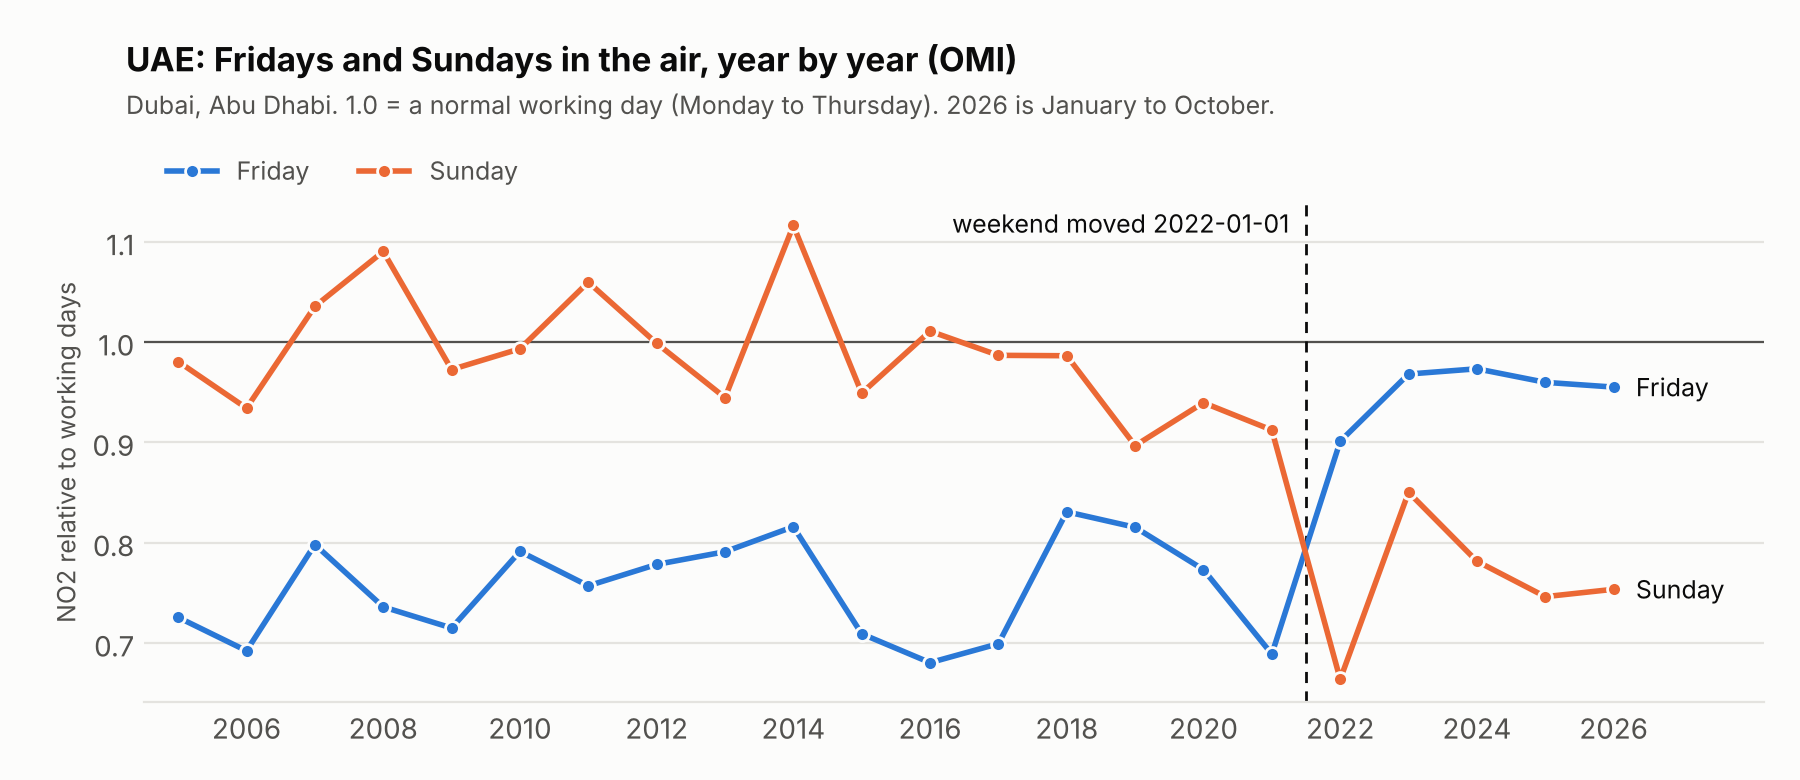
\includegraphics[width=\linewidth]{figures/UAE_2022_yearly.png}
  \caption{UAE: nitrogen dioxide on Fridays and Sundays relative to working days, year by year (OMI). The quietest day
  moves from Friday to Sunday in 2022.}
  \label{fig:uae}
\end{figure}

\subsection{What we tested and did not find}
In total we ran 81 pre-registered tests. Everything that would have made the water results surprising came back not
shown: more water stored than rain minus evaporation explains, slower draining than usual, a darker desert surface
afterwards, a change in Morocco's winter recharge, and 14 long-term drifts across Africa tested on years no agent had
seen. A worldwide GRACE scan for record seasons examined 1{,}534 block-seasons; 97 were records on both solutions, fewer
than the about 148 expected by chance, and none of its five candidates was confirmed on SMAP (one supported, three not
shown, one could not be tested). Twice during development the harness called a textbook result ``new''; we caught it,
fixed the novelty check and logged the failure.

% ---------------------------------------------------------------------------------------------------------------
\section{Reproducibility}
The code, data bundles and registrations are public. One command, \texttt{python -m synaptic reproduce}, recomputes every
reported number offline from the saved evidence bundles (8 of 8 pass), and the test suite has 39 passing tests,
including checks that the trend test keeps its false-positive rate near 5\% on synthetic series with carry-over. Each
registration file holds the registered text, then the results exactly as they came out, then any deviations.

% ---------------------------------------------------------------------------------------------------------------
\section{Limitations}
\begin{itemize}
  \item GRACE resolves regions of roughly 300\,km and larger; the volumes are for large regions, not towns or dams.
        The two GRACE solutions disagree on the central Sahara (46 versus 73\,km$^3$), and the full uncertainty is wider
        than the range between solutions (for example 43--108\,km$^3$ for Lake Chad).
  \item SMAP measures only the top 5\,cm of soil and has 11 seasons, which limits the power of its checks.
  \item OMI passes at about 13:30 local time, so the weekend result reflects morning and midday activity.
  \item ``Not shown'' and ``not detected'' mean not significant; they do not prove the absence of a change.
  \item The agents are language models and make mistakes. The design does not make them right; it stops their
        mistakes from becoming claims.
  \item The application currently runs on the user's computer; a hosted version is future work.
\end{itemize}

% ---------------------------------------------------------------------------------------------------------------
\section{Use of artificial intelligence}
We disclose every use of AI. \textbf{In the product}, NVIDIA Nemotron models play the research agents; they propose,
and code decides. \textbf{To build the project}, an AI coding assistant (Claude, by Anthropic, through Claude Code)
wrote and revised parts of the code, ran analyses and the confirmation scripts under the team's direction, and drafted
documentation and this paper, which the authors reviewed. \textbf{Figures}~\ref{fig:app}--\ref{fig:ladder} are
illustrations made with AI assistance in the PaperBanana style and are labelled as such; all data figures are plotted from NASA data
by code in the repository. The research question, the design choices and the decisions about what to claim are the
team's.

% ---------------------------------------------------------------------------------------------------------------
\section{Conclusion}
Synaptic shows that an AI research group can search NASA Earth data at scale without over-claiming, if the agents are
only allowed to propose and code holds the power to decide. The same discipline powers a simple application in which
anyone can test a trend and get an honest answer. Next, we want students, journalists and water agencies to test a
trend before they trust it, to hand confirmed leads to scientists, and to add more NASA and partner-agency data.

\paragraph{Links.} Code: \url{https://github.com/0x-type/Synaptic}. Story map: \url{https://arcg.is/1uOXai3}.

\sloppy
\paragraph{Data.} All data are NASA open data accessed with one Earthdata login: MERRA-2 (doi:10.5067/AP1B0BA5PD2K),
GPM IMERG V07 (doi:10.5067/GPM/IMERG/3B-MONTH/07), GLDAS Noah 2.1 (doi:10.5067/SXAVCZFAQLNO), MODIS Aqua MYD08\_M3
C6.1 (doi:10.5067/MODIS/MYD08\_M3.061), MODIS Aqua chlorophyll (doi:10.5067/AQUA/MODIS/L3M/CHL/2022.0), OMI OMNO2d v4
(doi:10.5067/AURA/OMI/DATA3407), AIRS3STM v7 (doi:10.5067/UBENJB9D3T2H), CERES EBAF-TOA Ed4.2.1, GRACE/GRACE-FO JPL
mascons RL06.3 (doi:10.5067/TEMSC-3JC634), GRACE/GRACE-FO NASA GSFC mascons RL06v2.0, SMAP SPL3SMP v009
(doi:10.5067/4XXOGX0OOW1S), and the NASA Giovanni, POWER and ADS services.

\begin{thebibliography}{9}\small
\bibitem{yoon2026} Yoon et al. Autonomous AI agents discover reverse transcriptases with tandem repeat arrays.
  Anthropic, 2026.
\bibitem{gottweis2026} J.~Gottweis et al. Accelerating scientific discovery with Co-Scientist. \emph{Nature}, 2026.
  doi:10.1038/s41586-026-10644-y.
\bibitem{ntrs2009} Time-series analysis of remotely-sensed SeaWiFS chlorophyll in river-influenced coastal regions.
  NASA Technical Reports Server, NTRS 20090042747.
\bibitem{sen1968} P.~K.~Sen. Estimates of the regression coefficient based on Kendall's tau. \emph{Journal of the
  American Statistical Association}, 63:1379--1389, 1968.
\bibitem{mann1945} H.~B.~Mann. Nonparametric tests against trend. \emph{Econometrica}, 13:245--259, 1945.
\bibitem{kendall1975} M.~G.~Kendall. \emph{Rank Correlation Methods}. Griffin, London, 1975.
\bibitem{holm1979} S.~Holm. A simple sequentially rejective multiple test procedure. \emph{Scandinavian Journal of
  Statistics}, 6:65--70, 1979.
\end{thebibliography}

\end{document}
